\chapter{Integración compleja}

Las funciones reales están definidas sobre conjuntos de números reales y con frecuencia se integran sobre intervalos. Las funciones complejas están definidas sobre conjuntos de puntos en el plano complejo y se integran sobre curvas. Antes de definir esta integral, es conveniente tener claro los conceptos de curvas paramétricas en el plano real y la integral de línea real (ver capítulo \ref{chpt:recordatorios}).

\section{Curvas paramétricas en el plano}

Si bien en la sección \ref{sec:1_curvas_y_regiones_en_el_plano_complejo} dimos una noción de lo que son las curvas y las regiones en el plano complejo para definir el dominio de una función compleja, en esta sección vamos a profundizar un poco sobre los conceptos de curvas cerradas, abiertas, suaves, entre otras propiedades que pueden tener. 

Una curva en el plano complejo es una función $\Gamma :[a,b]\to\mathbb{C}$, definida en un intervalo real $[a,b]$ y que toma valores complejos\footnote{$\Gamma$: letra griega Gamma mayúscula.}. Para cada número $t$ en $[a,b]$, $\Gamma(t)$ es un número complejo, o un punto en el plano. El lugar geométrico de tales puntos es la gráfica de la curva. Sin embargo, la curva es más que un lugar geométrico de puntos en el plano. $\Gamma$ tiene una orientación natural, que es la dirección en la que el punto $\Gamma(t)$ se mueve a lo largo de la gráfica conforme $t$ crece de $a$ a $b$. En este sentido, es natural referirse a $\Gamma(a)$ como el \textit{punto inicial} de la curva y a $\Gamma(b)$ como el \textit{punto final}.

Si $\Gamma(t)=x(t)+jy(t)$, entonces la gráfica de $\Gamma$ es el lugar geométrico de los puntos $(x(t),y(t))$ para $a\leqslant t\leqslant b$. El punto inicial de $\Gamma$ es $(x(a),y(a))$ y el punto final es $(x(b),y(b))$ y $(x(t),y(t))$ se mueve del punto inicial al punto final conforme varía $t$ de $a$ a $b$. Las funciones $x(t)$ e $y(t)$ son todas las \textit{funciones coordenadas} de $\Gamma$.

\begin{example}
  Sea $\Gamma (t) = 2t + jt^2$ para $0\leqslant t\leqslant 2$. Entonces:
  $$
  \Gamma (t)=x(t)+jy(t),
  $$
  donde $x(t)=2t$ y $y(t)=t^2$. La gráfica de esta curva es la parte de la parábola $y=(x/2)^2$, que se muestra en la figura \ref{fig:ejemplo_parabola_gamma}.
    \begin{figure}[ht]
    \centering
    \begin{tikzpicture}[scale=0.7,>=stealth]
      % Ejes y grid
      \draw[step=1cm,gray,loosely dotted] (-0.2,-0.2) grid (4.5,4.5);
      \draw[->] (-0.5,0) -- (4.5,0) node[right] {\footnotesize$x(t)$};
      \draw[->] (0,-0.5) -- (0,4.5) node[above] {\footnotesize$y(t)$};
      \node[below left] at (0,0) {\scriptsize0};
      \foreach \i in {1,...,4}
        {
          \node[below] at (\i,0) {\scriptsize\i}; 
          \node[left] at (0,\i) {\scriptsize\i}; 
        }
      % Curva parabólica 
      \begin{scope}[very thick,decoration={
        markings,
        mark=at position 0.5 with {\arrow{>}}}
        ] 
        \draw[red,>->,postaction={decorate}] (0,0) parabola (4,4) node[above right] {$\Gamma(t)$};
      \end{scope}
      \end{tikzpicture}
    \caption{Gráfica de la curva $\Gamma (t) = 2t + jt^2$, $0\leqslant t\leqslant 2$.}
    \label{fig:ejemplo_parabola_gamma}
  \end{figure}

  Conforme $t$ varía de $0$ a $2$, el punto $\Gamma (t)=(2t,t^2)$ se mueve a lo largo de esta gráfica del punto inicial $\Gamma(0)=(0,0)$ al punto final $\Gamma(2)=(4,4)$. Las flechas indican esta orientación.
\end{example}

\begin{example}
  Sea $\Gamma(t)=e^{jt}$ para $0\leqslant t \leqslant 3\pi$. Entonces $\Gamma(t)=\cos(t)+j\sin(t)=x(t)+jy(t)$, así
  \begin{equation*}
    x(t)=\cos(t),\qquad y(t)=\sin(t)
  \end{equation*}
  Como $x^2+y^2=1$, todo punto en esta curva está en el círculo unitario alrededor del origen. Sin embargo, el punto inicial de $\Gamma$ es $\Gamma(0)=1$ y el punto final es $\Gamma(3\pi)=e^{j3\pi}=-1$. Esta curva no es cerrada. Si esta fuera una pista de carreras, la carrera empezaría en el punto 1 de la figura \ref{fig:ejemplo_circunferencia_abierta_gamma} y terminaría en $-1$. 
    \begin{figure}[ht]
    \centering
    \begin{tikzpicture}[scale=1.5,>=stealth]
      % Ejes y grid
      \draw[step=0.5cm,gray,loosely dotted] (-1.9,-1.4) grid (1.9,1.4);
      \draw[->] (-2,0) -- (2,0) node[right] {\footnotesize$x(t)$};
      \draw[->] (0,-1.5) -- (0,1.5) node[above] {\footnotesize$y(t)$};
      % leyenda de números de ejes
      \node[below left] at (0,0) {\scriptsize0};
      % eje x
      \node[below] at (0.5,0) {\scriptsize$\frac{1}{2}$}; 
      \node[below right] at (1,0) {\scriptsize $\Gamma(0)=1$}; 
      \node[below] at (-0.5,0) {\scriptsize$-\frac{1}{2}$}; 
      \node[below left] at (-1,0) {\scriptsize $\Gamma(3\pi)=-1$}; 
      % eje y
      \node[left] at (0,0.5) {\scriptsize$\frac{1}{2}$}; 
      \node[above left] at (0,1) {\scriptsize 1}; 
      \node[left] at (0,-0.5) {\scriptsize$-\frac{1}{2}$}; 
      \node[below left] at (0,-1) {\scriptsize -1}; 

      \begin{scope}[very thick,decoration={
        markings,
        mark=at position 0.2 with {\arrow{>}},
        mark=at position 0.6 with {\arrow{>}},
        mark=at position 0.9 with {\arrow{>}},
      }] 
        \draw[red,postaction={decorate}] (0,0) circle (1);
      \end{scope}
      
      \coordinate (A) at (1,0);
      \coordinate (B) at (-1,0);
      \coordinate (C) at (45:1);
      \foreach \point in {A,B,C}
        \fill [black,opacity=.5] (\point) circle (2pt);
      \node[above right] at (C) {\scriptsize$\Gamma(t)=e^{jt}$};
    \end{tikzpicture}
    \caption{$\Gamma(t)=e^{jt}$ para $0\leqslant t\leqslant 3\pi$.}
    \label{fig:ejemplo_circunferencia_abierta_gamma}
  \end{figure}

  Una pista de carreras circular no significa que los puntos de inicio y fin de la carrera sean el mismo. Esto no es evidente a partir sólo de la gráfica. $\Gamma$ está orientada positivamente, como lo indica la flecha.
  \label{ej:circunferencia_abierta}
\end{example}
\begin{example}
  Si se tomase el mismo caso que el ejemplo \ref{ej:circunferencia_abierta}, pero ahora el intervalo es $0\leqslant t \leqslant 4\pi$, resulta que ahora la curva si es cerrada, sin embargo $\Gamma(t)$ se mueve alrededor del círculo unitario dos veces conforme $t$ varía en el intervalo.
  \label{ej:circunferencia_cerrada_no_simple}
\end{example}

Una curva $\Gamma$ es \textit{simple} si $\Gamma(t_1)\neq \Gamma(t_2)$ siempre que $t_1\neq t_2$. Esto significa que el mismo punto nunca se repite en tiempos diferentes. Se hace una excepción para las curvas cerradas, que requieren que $\Gamma(a)=\Gamma(b)$. Si éste es el único punto en el cual $\Gamma(t_1)=\Gamma(t_2)$ con $t_1\neq t_2$, entonces $\Gamma$ es una \textit{curva cerrada simple}. La curva del ejemplo \ref{ej:circunferencia_cerrada_no_simple} es una curva cerrada, pero no simple. Si se define otra curva, igual a la del ejemplo \ref{ej:circunferencia_cerrada_no_simple} pero el intervalo es $0\leqslant t \leqslant 2\pi$, entonces $\Gamma$ es una curva cerrada simple.

Una curva $\Gamma:[a,b]\to \mathbb{C}$ es \textit{continua} si cada una de sus funciones coordenadas es continua en $[a,b]$. Si $x(t)$ y $y(t)$ son diferenciables en $[a,b]$, $\Gamma$ es una \textit{curva diferenciable}. Si $x'(t)$ y $y'(t)$ son continuas, y no valen cero para el mismo valor de $t$, $\Gamma$ es una \textit{curva suave}. Todas las curvas de los ejemplos anteriores son suaves.

En términos vectoriales, se puede escribir como $\Gamma(t)=x(t)\hat{\imath} + y(t)\hat{\jmath}$ como se ha visto en el capítulo \ref{chpt:recordatorios}. Si $\Gamma$ es diferenciable, y $x'(t)$ y $y'(t)$ no son cero, entonces $\Gamma'(t)=x'(t)\hat{\imath}+y'(t)\hat{\jmath}$ es el vector tangente a la curva en el punto $\Gamma(t)$ (figura \ref{fig:vector_tangente_a_una_curva}). Si $\Gamma$ es suave, entonces las derivadas $x'(t)$ y $y'(t)$ son continuas, así que el vector tangente es continuo (se puede encontrar un único $\Gamma'$ para cada punto de la curva).

\begin{figure}[ht]
  \centering
  \begin{subfigure}[b]{0.48\textwidth}
    \centering
    \begin{tikzpicture}[>=stealth]
      % Ejes
      \draw[->] (-1,0) -- (3,0) node[right] {\footnotesize$x$};
      \draw[->] (0,-0.5) -- (0,1.5) node[above] {\footnotesize$y$};

      \begin{scope}[very thick,decoration={
        markings,
        mark=at position 0.3 with {\arrow{>}},
        mark=at position 0.5 with {
          \coordinate (G) at (0,0);
          \draw[->,black,opacity=.7] (0,0) -- (1,0) node[right] {\footnotesize$\Gamma'(t)$}; 
        },
      }] 
        \draw[red,postaction={decorate}] (-0.9,-0.4) .. controls (0,1.2) and (0.9,1.4) .. (2.8,1);
      \end{scope}
      \fill [black,opacity=.5] (G) circle (2pt);
      \draw[->,very thick,black,opacity=.7] (0,0) -- (G) node[below right] {$\Gamma(t)$};
    \end{tikzpicture}
    \caption{Vector tangente a una curva.}
    \label{fig:vector_tangente_a_una_curva}
  \end{subfigure}
  \hfill
  \begin{subfigure}[b]{0.48\textwidth}
    \centering
    \begin{tikzpicture}[>=stealth]
      % Ejes
      \draw[->] (-1.5,0) -- (2.5,0) node[right] {\footnotesize$x$};
      \draw[->] (0,-0.5) -- (0,1.5) node[above] {\footnotesize$y$};

      \coordinate (A) at (-1.4,0.5);
      \coordinate (B) at (0.3,1);
      \begin{scope}[very thick,decoration={
        markings,
        mark=at position 0.3 with {\arrow{>}},
        mark=at position 0.5 with {
          \node[above] {\scriptsize$\Gamma_1$};
        },
      }] 
        \draw[red,postaction={decorate}] (A) .. controls (-0.9,0.9) and (-0.4,1.1) .. (B);
      \end{scope}
      \coordinate (C) at (0.6,0.2);
      \node[red,fill=white] at (0,0.6) {\scriptsize$\Gamma_2$};
      \begin{scope}[very thick,decoration={
        markings,
        mark=at position 0.5 with {\arrow{>}},
      }] 
        \draw[red,postaction={decorate}] (B) .. controls (0.35,0.5) .. (C);
      \end{scope}
      \coordinate (D) at (1.3,1.3);
      \begin{scope}[very thick,decoration={
        markings,
        mark=at position 0.5 with {\arrow{>}},
        mark=at position 0.6 with {
          \node[above=5pt] {\scriptsize$\Gamma_3$};
        }
      }] 
        \draw[red,postaction={decorate}] (C) .. controls (0.7,0.6) and (0.9,1) .. (D);
      \end{scope}
      \coordinate (E) at (2.4,-0.4);
      \begin{scope}[very thick,decoration={
        markings,
        mark=at position 0.4 with {\arrow{>}},
        mark=at position 0.5 with {
          \node[right] {\scriptsize$\Gamma_4$};
        }
      }] 
        \draw[red,postaction={decorate}] (D) .. controls (1.9,1.2) and (2,-0.4) .. (E);
      \end{scope}

      \foreach \i in {A,B,C,D,E} 
        \fill [gray] (\i) circle (2pt);
    \end{tikzpicture}
    \caption{La \textit{concatenación}.}
    \label{fig:curva_a_trozos}
  \end{subfigure}
\end{figure}


A veces se forma una curva $\Gamma$ juntando varias curvas $\Gamma_1,\dots, \Gamma_n$ en sucesión. Es importante que, el punto final de $\Gamma_{k-1}$ debe ser el mismo que el punto inicial de la siguiente curva $\Gamma_k$ para $k=1,\dots,n$ (figura \ref{fig:curva_a_trozos}). Una curva así se llama la \textit{concatenación} de $\Gamma_1,\dots,\Gamma_n$. Las curvas $\Gamma_k$ son las \textit{componentes} de esta concatenación. Si cada componente de una concatenación es suave, entonces es una curva \textbf{suave a trozos}. Tiene una tangente continua en cada punto, excepto quizá en los puntos de conexión entre curvas. Si la conexión es de manera suave (como sucede en la conexión entre $\Gamma_3$ y $\Gamma_4$ en la figura \ref{fig:curva_a_trozos}), la concatenación puede tener una tangente en cada uno de estos puntos y ella misma ser suave. En otras palabras, cuando la conexión entre dos curvas es suave, puede existir la derivada en la conexión, y ser tratada como una curva suave completa (y no suave a trozos).


\section{La integral compleja}

\begin{definition}
Sea $f$ una función compleja y $\Gamma:[a,b]\to\mathbb{C}$ una curva suave en el plano. Suponiendo que $f$ es continua en todos los puntos de $\Gamma$, entonces la integral de $f$ sobre $\Gamma$ se define como
$$
\int_\Gamma f(z)\,dz = \int_a^b f(\Gamma(t))\Gamma'(t)\,dt
$$
Como $z=\Gamma(t)$ en la curva, esta integral se escribe frecuentemente como
$$
\int_\Gamma f(z)\,dz = \int_a^b f(z(t))z'(t)\,dt
$$
Esta formulación tiene la ventaja de sugerir la manera que $\int_\Gamma f(z)dz$ es evaluada. Reemplazando $z$ con $z(t)$ en la curva y encontrando la expresión $dz=z'(t)dt$ sobre el intervalo $a\leqslant t\leqslant b$. 
\end{definition}


\section{Teorema de Cauchy}

El teorema de Cauchy (o integral de Cauchy) es considerado el teorema fundamental de la integración compleja. El enunciado del teorema usa implícitamente el teorema de la curva de Jordan, que establece que una curva continua, simple y cerrada en el plano separa al plano en dos conjuntos abiertos. Uno de estos conjuntos es no acotado y se llama el \textit{exterior}, y el otro es acotado y se llama el \textit{interior}. La curva misma no pertenece a ninguno de estos conjuntos, pero marca la frontera de ambos.

\begin{figure}[ht]
  \centering
  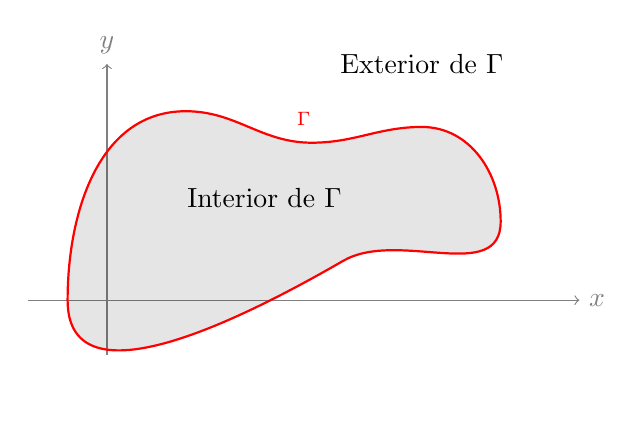
\begin{tikzpicture}
    \draw[->,gray] (-1,0) -- (6,0) node[right] {$x$};
    \draw[->,gray] (0,-0.7) -- (0,3) node[above] {$y$};

    \draw[thick,red,fill=black,fill opacity=0.1] (-0.5,0) to [out=90,in=180] (1,2.4)
    to [out=0,in=180] (2.6,2) 
    to [out=0,in=180] (4,2.2)
    to [out=0,in=90] (5,1)
    to [out=-90,in=30] (3,0.5)
    to [out=210,in=-90] (-0.5,0);
    \node[red] at (2.5,2.3) {\scriptsize$\Gamma$};

    \node at (2,1.3) {Interior de $\Gamma$};
    \node at (4,3) {Exterior de $\Gamma$};
  \end{tikzpicture}
  \caption{Teorema de la curva de Jordan.}
\end{figure}

A pesar de que esta conclusión puede parecer obvia para las curvas cerradas que se suelen dibujar, es difícil de probar debido a la generalidad de su enunciado. 

En la sección \ref{sec:1_curvas_y_regiones_en_el_plano_complejo} estuvimos analizando algunas regiones del plano complejo y sus propiedades. Esto lo hicimos para poder definir el dominio de una función compleja. Ahora vamos a profundizar algunos aspectos sobre las regiones del plano complejo para poder enunciar correctamente el teorema de Cauchy.

\begin{definition}[Trayectoria]
  Una trayectoria es una curva simple, suave a trozos. Una trayectoria pertenece a un conjunto $S$ si su gráfica está contenida dentro de $S$
\end{definition}

Algunas de las curvas paramétricas que hemos realizado anteriormente (como la figura \ref{fig:ejemplo_parabola_gamma}) son trayectorias en $\mathbb{C}$. Así, una trayectoria es una concatenación de curvas suaves que no se cruzan a sí mismas.

\begin{definition}[Conjunto conexo]
  Un conjunto $S$ de números complejos es conexo si, dados dos puntos cualesquiera de $z$ y $w$ en $S$, existe una trayectoria en $S$ que tiene a $z$ y a $w$ como puntos extremos.
\end{definition}

$S$ es conexo si es posible ir desde cualquier punto de $S$ a cualquier otro punto moviéndose a lo largo de alguna trayectoria totalmente contenida en $S$. Un disco abierto es conexo, así como también lo es un disco cerrado (ver sección \ref{sec:1_curvas_y_regiones_en_el_plano_complejo}).

\begin{definition}[Dominio]
  Como ya hemos visto, un conjunto de números complejos, abierto y conexo se llama dominio.
\end{definition}

\begin{definition}[Simplemente conexo]
  Un conjunto $S$ de números complejos es simplemente conexo si toda trayectoria cerrada en $S$ encierra únicamente puntos de $S$.
\end{definition}

Todo disco abierto es simplemente conexo. Si dibuja una trayectoria cerrada en un disco abierto, esta trayectoria cerrada encerará solamente puntos en el disco abierto. El anillo o corona de la figura \ref{fig:corona_complx} no es simplemente conexo. A pesar de ser conexo, se puede dibujar una trayectoria cerrada contenida en el anillo que encierra puntos que no pertenecen al anillo (son aquellos puntos excluidos por la frontera interna).

Ahora si, estamos listos para enunciar el teorema de Cauchy.

\subsection[Enunciado del teorema]{El teorema de Cauchy}

\begin{theorem}[Teorema de Cauchy]
  Sea $f$ diferenciable en un dominio simplemente conexo $G$. Sea $\Gamma$ una trayectoria cerrada en $G$. Entonces
  \[
    \oint_\Gamma f(z)dz=0
  \]
\end{theorem}

